%; whizzy chapter
% -initex iniptex -latex platex -format platex -bibtex jbibtex -fmt fmt
% 以上 whizzytex を使用する場合の設定。

%     Tokyo Debian Meeting resources
%     Copyright (C) 2011 Junichi Uekawa
%     Copyright (C) 2011 Nobuhiro Iwamatsu

%     This program is free software; you can redistribute it and/or modify
%     it under the terms of the GNU General Public License as published by
%     the Free Software Foundation; either version 2 of the License, or
%     (at your option) any later version.

%     This program is distributed in the hope that it will be useful,
%     but WITHOUT ANY WARRANTY; without even the implied warranty of
%     MERCHANTABILITY or FITNESS FOR A PARTICULAR PURPOSE.  See the
%     GNU General Public License for more details.

%     You should have received a copy of the GNU General Public License
%     along with this program; if not, write to the Free Software
%     Foundation, Inc., 51 Franklin St, Fifth Floor, Boston, MA  02110-1301 USA

%  preview (shell-command (concat "evince " (replace-regexp-in-string "tex$" "pdf"(buffer-file-name)) "&"))
% 画像ファイルを処理するためにはebbを利用してboundingboxを作成。
%(shell-command "cd image201201; ebb *.png")

%%ここからヘッダ開始。

\documentclass[mingoth,a4paper]{jsarticle}
\usepackage{monthlyreport}

% 日付を定義する、毎月変わります。
\newcommand{\debmtgyear}{2012}
\newcommand{\debmtgmonth}{2}
\newcommand{\debmtgdate}{18}
% (+ (* (- 2012 2005) 12) 1 -1) started from zero
\newcommand{\debmtgnumber}{0}

\begin{document}

\begin{titlepage}
\thispagestyle{empty}
% タイトルページ:編集必要な部分は最初のマクロに飛ばすこと

\vspace*{-2cm}
第\debmtgnumber{}回 福岡 Debian 勉強会資料\\
\hspace*{-2cm}
\includegraphics[width=210mm]{image201003/debsen.eps}\\
\hfill{}\debmtgyear{}年\debmtgmonth{}月\debmtgdate{}日

% ここはアップデートすること
% 全角文字にしないとフォントのサイズが合わないので注意
\rotatebox{10}{\fontsize{32}{32} {\gt 特集1: XXXX}}

\rotatebox{10}{\fontsize{32}{32} {\gt 特集2: YYYY}}

\vspace*{-2cm}
\hfill{}
\includegraphics[height=6cm]{image200502/openlogo-nd.eps}
\end{titlepage}

\dancersection{Introduction}{岩松 信洋}

\begin{multicols}{2}
 

 今月のDebian勉強会へようこそ。これからDebianの世界にあしを踏み入れると
 いう方も、すでにどっぷりとつかっているという方も、月に一回Debianについ
 て語りませんか?

 Debian勉強会の目的は下記です。

 \begin{itemize}
 \item \underline{Debian Developer} (開発者)の育成。
 \item 日本語での「\underline{開発に関する情報}」を整理してまとめ、アップデートする。
 \item \underline{場}の提供。
 \begin{itemize}
  \item 普段ばらばらな場所にいる人々が face-to-face で出会える場を提供
	する。
  \item Debian のためになることを語る場を提供する。
  \item Debianについて語る場を提供する。
 \end{itemize}
 \end{itemize}		

 Debianの勉強会ということで究極的には参加者全員がDebian Packageをがりがり
 と作るスーパーハッカーになった姿を妄想しています。情報の共有・活用を通し
 て Debianの今後の能動的な展開への土台として、「場」としての空間を提供す
 るのが目的です。

\end{multicols}

\newpage

\begin{minipage}[b]{0.2\hsize}
 \definecolor{titleback}{gray}{0.9}
 \colorbox{titleback}{\rotatebox{90}{\fontsize{80}{80} {\gt デビアン勉強会} }}
\end{minipage}
\begin{minipage}[b]{0.8\hsize}
\hrule
\vspace{2mm}
\hrule
\begin{multicols}{2}
\tableofcontents
\end{multicols}
\vspace{2mm}
\hrule
\end{minipage}

\dancersection{事前課題}{岩松 信洋}

今回の事前課題は以下です:
\begin{enumerate}
 \item 2012年の勉強会のテーマとして各月なにをするべきか提案してくさい。 
 \item 自分がどのテーマを担当したいか提案してください。
\end{enumerate}
この課題に対して提出いただいた内容は以下です。
\begin{multicols}{2}
{\small
% %; whizzy-master ../debianmeetingresume201201.tex
% 以上の設定をしているため、このファイルで M-x whizzytex すると、
% whizzytexが利用できます

\begin{prework}{上川 純一}

テーマ案です。

\begin{itemize}
 \item Android/iOSをDebianから使う (USB device driver, wifi, bluetooth,
       adb などなど)
 \item 電話でdebianを使う
 \item タブレットでDebianを使う
 \item Debianからクラウドサービスを使う (EC2 API とか)
 \item ウェブアプリケーション開発をDebianでする
 \item Debianのウェブブラウザ
 \item nodejs
 \item Debianでのjavascriptの開発・パッケージ
 \item clojure / Debian
\end{itemize}
 
\end{prework}

\begin{prework}{まえだこうへい}

\begin{itemize}
  \item DebianでOpenStack
  \item Python2, 3、両方に対応したパッケージ作成
  \item Pythonのテストツール
  \item Vyattaネタ(Debianベース、という意味で)
  \item webOSネタ(Ubuntuベース、という意味で)
\end{itemize}

\end{prework

% TODO: paste prework here.

}
\end{multicols}

\dancersection{最近のDebian関連のミーティング報告}{岩松 信洋}
\subsection{東京エリアDebian勉強会84回目報告}

% (query-replace-regexp "<.*?>" "")
% (query-replace-regexp "^[	 ]\+" "")



\dancersection{Debian Trivia Quiz}{岩松 信洋}

ところで、みなさん Debian 関連の話題においついていますか?Debian関連の話
題はメーリングリストをよんでいると追跡できます。ただよんでいるだけではは
りあいがないので、理解度のテストをします。特に一人だけでは意味がわからな
いところもあるかも知れません。みんなで一緒に読んでみましょう。

今回の出題範囲は\url{debian-devel-announce@lists.debian.org} や \url{debian-devel@lists.debian.org}に投稿された
内容とDebian Project Newsからです。

\begin{multicols}{2}
% %; whizzy-master ../debianmeetingresume201211.tex
% $B0J>e$N@_Dj$r$7$F$$$k$?$a!"$3$N%U%!%$%k$G(B M-x whizzytex $B$9$k$H!"(Bwhizzytex$B$,MxMQ$G$-$^$9!#(B
%

\santaku
{DebConf13 $B$N3+:ECO$H3+:EF|$O!)(B}
{$BF|K\!"El5~ET(B 6$B7n(B20$BF|(B}
{$B%K%+%i%0%"(B $B%^%J%0%"(B 7$B7n(B8-14$BF|(B}
{$B%9%$%9!"%t%)!<%^%k%-%e(B 8$B7n(B11-18$BF|(B}
{3}
{$B%K%+%i%0%"$O(BDebConf12$B$N3+:ECO$G$9!#(B
DebConf13$B$O%9%$%9$N%-%c%s%WCO$G3+:E$G$9!#(B
6/20$B$O3'$5$sM=Dj$r6u$1$F$*$-$^$7$g$&!#(B}

\santaku
{$B@$3&$N(BWeb$B%5!<%P$G:G$b?M5$$N$"$k(BLinux $B%G%#%9%H%j%S%e!<%7%g%s(B(W3Techs$BD4$Y(B)$B$O!)(B}
{CentOS}
{Debian}
{Ubuntu}
{B}
{\url{http://w3techs.com/technologies/history_details/os-linux}$B$K7k2L$N%0%i%U$,$"$j$^$9!#(B
$B8=:_(B Linux $B$r;HMQ$7$F$$$k(B web $B%5!<%P$N(B 32.9\% $B$,(B Debian $B$rMxMQ$7$F$*$j!"$=$N3d9g$O8=:_$bA}2C$rB3$1$F$$$k$=$&$G$9!#(B}

\santaku
{Debian $B%+!<%M%k%A!<%`$N%a%s%P!<$G$"$j!"(Bkernel.org $B$N(B 3.2.y $B0BDjHG7ONs$N%a%s%F%J$G$b$"$k(B Ben Hutchings $B$5$s$,<!4|(B Debian $B0BDjHG$H0l=o$K=P2Y$5$l$k(B Linux $B%+!<%M%k$K(B (3.2 $B7ONs$N(B mainline $B$K$OL5$$(B) $BDI2C5!G=$,Ek:\$5$l$kM=Dj$G$"$k$H=R$Y$F$$$^$9!#(B
$BB?$/$NDI2CE@$NCf$K4^$^$l$J$$$b$N$O2?!)(B}
{PREEMPT\_RT}
{Hyper-V guest drivers$B$N6/2=(B}
{ARM64/AArch64$B%"!<%-%F%/%A%c%5%]!<%H(B}
{C}
{Hyper-V guest drivers$B$O(Bmainline kernel$B$G(B3.2$B$K$b4^$^$l$F$$$^$9$,!"$h$j2~A1$5$l$?(B3.4$B$+$i$N=$@5$,F3F~$5$l$^$9!#(B
PREEMPT\_RT$B$O%O!<%I%j%"%k%?%$%`$r<B8=$9$k$?$a$N(BPatch$B!"(B
linux-image-rt-amd64 , linux-image-rt-686-pae $B$N(Bmetapackage$B$G;HMQ$G$-$^$9!#(B
$B?7$7$$(BARM 64$B%S%C%H%"!<%-%F%/%A%c%5%]!<%H$O(Bmainline kernel 3.7$B$+$i(B}

\santaku
{Wookey$B$5$s$,%"%J%&%s%9$7$?(Balpha$BHG$N(BDebian port arm64 image$B$O!)(B}
{Debian/Ubuntu port image}
{Debian/KFreeBSD port image}
{Debian/GnuHurd port image}
{A}
{self-bootstrapp(non x86)$BBP1~$H$N$3$H$G$9!#(B\url{http://wiki.debian.org/Arm64Port}$B$G%9%F!<%?%9$,3NG'$G$-$^$9!#(B}

\santaku
{700,000$BHVL\$N%P%0$,Js9p$5$l$?F|$rEv$F$k(B700000thBugContest$B$N7k2L$,=P$^$7$?!#$=$NM=A[F|$HJs9pF|$O!)(B}
{2012/12/12$B$rM=A[$7$?(BDavidPrevot}
{$BM=A[F|(B:2013/02/04$B!"Js9pF|(B:2013/02/14}
{$BM=A[F|(B:2013/02/07$B!"Js9pF|(B:2013/02/14}
{$BM=A[F|(B:2013/02/14$B!"Js9pF|(B:2013/02/07}
{C}
{$B:G$b6a$$(B2013/02/14$B$rM=A[$7$?(BChristian Perrier$B$5$s$,Ev$F$^$7$?!#7k2L$O(B\url{http://wiki.debian.org/700000thBugContest}$B$G8x3+$5$l$F$$$^$9!#(B
$B$^$?!"(B800,000/1,000,000$BHVL\$N%P%0$,Js9p$5$l$kF|$rEv$F$k%3%s%F%9%H(B\url{http://wiki.debian.org/800000thBugContest}$B$b3+:E$5$l$F$$$^$9!#(B}

\santaku
{master.debian.org$B$,?7$7$$5!3#$K0\9T$5$l$^$7$?!#$3$l$O2?$N%5!<%P$G$7$g$&$+(B $B!)(B}
{@debian.org$B$N%a!<%k%5!<%P(B}
{$B%Q%C%1!<%8$N%^%9%?!<%5!<%P(B}
{$B%Q%C%1!<%8$N%9%]%s%5!<(B(mentor)$B$rC5$9%5!<%P(B}
{A}
{$B8E$$%5!<%P$O%G%#%9%/>c32Ey$,$"$C$?$N$G!"<wL?$HH=CG$5$l!"%G!<%?$,B;<:$9$kA0$K?7$7$$%5!<%P$K0\9T$5$l$^$7$?!#(Bftp-master.debian.org$B$O(BDebian$B$N(B official package $B%j%]%8%H%j$G$9!#%Q%C%1!<%8$N%9%]%s%5!<(B(mentor)$B$rC5$9$N$O(Bmentors.debian.net$B!#(B }

\santaku
{pbuilder$B$K(Bclang support$B$,DI2C$5$l$^$7$?!#C/$,=q$$$?%Q%C%A$G$7$g$&$+!)(B}
{Sylvestre Ledru}
{Junichi Uekawa}
{Hideki Yamane}
{C}
{Debian$B$N(BClang$B%5%]!<%H$OCe!9$H?J$s$G$$$^$9!#(B}

\santaku
{DPN - 2013$BG/(B3$B7n(B4$BF|9f$K<h$j>e$2$i$l$?F|K\$N%$%Y%s%H$O(B}
{Open Source Conference 2013 Tokyo/Spring}
{Open Source Conference 2013 Hamamatu}
{Open Source Conference 2013 Tokushima}
{A}
{\url{http://henrich-on-debian.blogspot.jp/2013/02/open-source-conference-2013-tokyospring.html} $B>\:Y$O8e$[$I!#(B}


\end{multicols}

\dancersection{Dynamic Kernel Module Support Framework}{岩松 信洋}

\subsection{Dynamic Kernel Module Support Frameworkとは}

Dynamic Kernel Module Support Framework(以下、DKMS)は、
マシンにインストールされているカーネル毎に
自動的にドライバモジュールをビルドし管理する仕組みです。

通常、
Linuxカーネルが更新されたとき、Linuxカーネルで提供されていない
サードパーティのドライバはそのLinuxカーネル用にデバイスドライバを
再ビルドおよびインストールを行う必要があります。
しかし DKMS を使ってサードパーティのデバイスドライバを管理している場合、
新しいLinuxカーネルで起動された時に対応したデバイスドライバがないことを
チェックし、ドライバモジュールをビルドして
(自動インストールが設定されていれば)インストールします。
もちろんそのドライバはLinuxカーネルに対応している必要がありますが、
ドライバがメンテナンスされていれば、半自動的に新しいカーネルへ移行
できるようになります。

\if 0
メリットが大きい DKMS ですが、起動時にビルドする
ので、規模が大きいドライバモジュールでは起動に時間がかかるという
デメリットもあります。
\fi

DKMS は DELL \url{http://linux.dell.com/dkms/} で開発されており、
DebianやUbuntuなどののディストリビューションで利用できるようになって
います。

ちなみに Fedora は
Kmods2 \url{http://rpmfusion.org/Packaging/KernelModules/Kmods2} と呼ばれる
別のフレームワークを利用しています。Arch Linux と Gentoo も DKMS サポート
パッケージもあるが、独自の実装が中心のようです。

今回は DKMS の仕組みと DKMS に対応したパッケージの作成方法、
Debian の DKMS 対応状況について説明します。

\subsection{DKMS の仕組み}

\begin{multicols}{2}

DKMS の仕組みを理解するために簡単なデバイスドライバを使って
説明します。ドライバをロードすると カーネルデバッグメッセージ
に「Hello, world! from hello\_init」、ドライバをアンロードすると
「Good bye! from hello\_exit」と出力するものです。
以下に実際のソースコード、Makefile、実行結果とディレクトリ構成を示します。

ドライバソースコード:
\begin{commandline}
#include <linux/init.h>
#include <linux/module.h>

static int __init hello_init(void)
{
  pr_info("Hello, world! from %s\n", __func__);
  return 0;
}

static void __exit hello_exit(void)
{
  pr_info("Good bye! from %s\n", __func__);
}

module_init(hello_init);
module_exit(hello_exit);
MODULE_LICENSE("GPL v2");
\end{commandline}
%$

Makefile:
\begin{commandline}
obj-m:= src/
\end{commandline}
%$

src/Makefile:
\begin{commandline}
obj-m:= hello.o 
\end{commandline}
%$


ドライバのコンパイルと実行結果:
\begin{commandline}
$ make -C /lib/modules/`uname -r`/build M=`pwd` modules
$ sudo insmod hello.ko
$ dmesg | tail -1
[5963787.044134] Hello, world! from hello_init
$ sudo rmmod hello.ko
$ dmesg | tail -1
[5963798.420368] Good bye! from hello_exit
\end{commandline}
%$

ディレクトリ構成:
\begin{commandline}
hello-0.0.1
├─Makefile
├── README
├── dkms.conf
└--src
    ├── Makefile
    └── hello.c
\end{commandline}

dkms.conf:
\begin{commandline}
PACKAGE_NAME="hello"
PACKAGE_VERSION="0.0.1"
BUILT_MODULE_NAME="$PACKAGE_NAME"
BUILT_MODULE_LOCATION="src"
DEST_MODULE_LOCATION="/updates"
AUTOINSTALL="yes"
\end{commandline}
%$

\end{multicols}

\subsubsection{DKMS 全体の流れ}

DKMS の全体の流れは以下のようになっています。
各要素はDKMS で提供されているコマンドとスクリプトになっています。

\begin{figure}[ht] 
 \begin{center}
  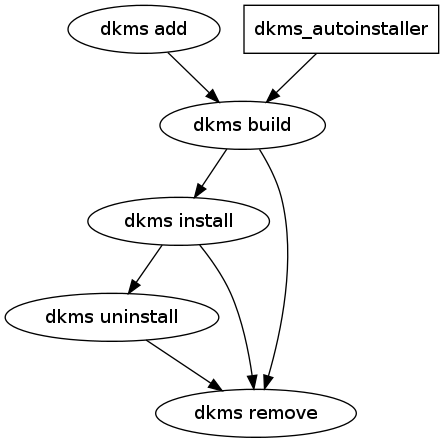
\includegraphics[width=0.4\hsize]{image201202/dkms.png}
 \end{center}
\label{fig:dkms}\caption{DKMS 全体の流れ}
\end{figure}

dkms\_autoinstaller はシステム起動時に呼ばれる
\footnote{ディストリビューションによって異なる}スクリプトです。
既に DKMS に登録(dkms add)されているドライバモジュールの中で、
現在起動しているカーネル用にドライバモジュールがインストール
(dkms install)されていないものがあれば、
ドライバモジュールのビルドとインストール
(dkms build / dkms install)が実行されます。

\subsubsection{モジュールソースコードの配置位置}

DKMS 対応モジュールのソースコードは
\url{/usr/src/ドライバモジュール名-バージョン/} 以下に配置する必要があります。
先のドライバの場合、\url{/usr/src/hello-0.0.1/} 以下に配置します。

\subsubsection{DKMS 設定ファイル}

DKMS は、各ドライバパッケージ毎に設定ファイルを持つ必要があります。
この設定ファイルでは、どのようなドライバが提供、ビルド、インストールされるのか
記述されている必要があります。以下によく利用する設定項目を示します。
\begin{table}[ht]
 \caption{DKMS 設定ファイル項目}
 \label{tab:dkms-config-file}
\begin{center}
  \begin{tabular}{|l|p{35zw}|}
 \hline
 設定項目 & 内容 \\
 \hline \hline
PACKAGE\_NAME & パッケージ名 \\
PACKAGE\_VERSION & パッケージバージョン \\
CLEAN & キャッシュなどの一時ファイルを削除するためのコマンドを指定する。指定しない場合には "make clean" が実行される。\\
MAKE & モジュールをビルドするコマンドを指定する。\\
BUILT\_MODULE\_NAME & ドライバモジュールの名前を指定する(拡張子は必要なし)。\\
BUILT\_MODULE\_LOCATION &  ビルドされたモジュールが作成されるディレクトリまでの相対パス\\
DEST\_MODULE\_LOCATION & モジュールをインストールするディレクトリを指定する。\\
AUTOINSTALL & モジュールを自動的にインストールするか、"yes" か "no" を指定する。\\
REMAKE\_INITRD & ドライバインストール時にINITRD イメージを再構成するか、"yes" か "no" を指定する。 \\
PATCH & 適用したいパッチを指定する。\\
PATCH\_MATCH & パッチを適用するバージョンの指定する。Linux カーネルが 2.6.38 と 2.6.39 の場合にパッチを適用したい場合には "2\.6\.(38|39)" と指定する。\\
 \hline
 \end{tabular}
\end{center}
\end{table}

BUILT\_MODULE\_LOCATION や BUILT\_MODULE\_NAME などは
配列を使ってドライバモジュール毎に設定できます。
BUILT\_MODULE\_NAME 配列の番号は各要素の番号に紐づいているので、
処理されるときは各々の番号が参照されます。
例えば、一つのドライバパッケージから foo と bar の2つのデバイスドライバ
が提供される場合、以下のように設定することができます。

\begin{commandline}
(省略)
BUILT\_MODULE\_NAME[0] = "foo"
BUILT\_MODULE\_LOCATION[0]  = "foo_build"
DEST\_MODULE\_LOCATION[0] = "/update"
BUILT\_MODULE\_NAME[1] = "bar"
BUILT\_MODULE\_LOCATION[1]  = "bar_build"
DEST\_MODULE\_LOCATION[1] = "/update"
(省略)
\end{commandline}

これにより、ドライバ foo のビルドは foo\_build ディレクトリで行われ、
update ディレクトリ以下にインストール、ドライバ bar のビルドは
bar\_build ディレクトリで行われ、update ディレクトリ以下にインストール
されます。

\subsubsection{DKMS で提供されるコマンド}
DKMS は dkms コマンドで操作します。
以下に利用頻度が高いコマンドを紹介します。

\begin{enumerate}
\item dkms status\\
DKMS で提供されている モジュールのステータスを表示します。
\begin{commandline}
$ dkms status
v4l2loopback, 0.5.0, 3.1.0-1-amd64, x86_64: installed
v4l2loopback, 0.5.0, 3.2.0-1-amd64, x86_64: installed
virtualbox, 4.1.8, 3.1.0-1-amd64, x86_64: installed
virtualbox, 4.1.8, 3.2.0-1-amd64, x86_64: installed
\end{commandline}
%$

\item dkms add \\
モジュールのソースコードを管理対象に追加します。
実行する時に -m オプションで追加するドライバパッケージ名を、
-v オプションでバージョンを指定します。

\begin{commandline}
$ sudo dkms add -m hello -v 0.0.1

Creating symlink /var/lib/dkms/hello/0.0.1/source ->
                 /usr/src/hello-0.0.1

DKMS: add completed.
$ dkms status
hello, 0.0.1: added
\end{commandline}
%$

実行すると/var/lib/dkms 以下に シンボリックリンクを張り、DKMS が管理する
ドライバデータベースに登録されます。

\item dksm build \\
管理対象になっているモジュールをビルドします。
実行する時に -m オプションで追加するドライバパッケージ名を、
-v オプションでバージョンを指定します。

ドライバは \url{/var/lib/dkms/ドライバ名/ドライババージョン/BUILT\_MODULE\_LOCATION} 以下
でビルドされます。                   
作成されたモジュールとビルドログは
\url{/var/lib/dkms/ドライバ名/ドライババージョン/カーネルバージョン/アーキテクチャ}
以下に置かれます。

\begin{commandline}
$ sudo dkms build -m hello -v 0.0.1

Kernel preparation unnecessary for this kernel.  Skipping...

Building module:
cleaning build area....
make KERNELRELEASE=3.0.0-1-amd64 -C /lib/modules/3.0.0-1-amd64/build M=/var/lib/dkms/hello/0.0.1/build....
cleaning build area....
\end{commandline}
% $

\item dksm install\\
dkms build コマンドによってビルドされたモジュールをdkms.conf の 
DEST\_MODULE\_LOCATION で指定されている場所にインストールします。
例えば Linux カーネル 3.2.0-1-amd64 を使っていて、
\begin{commandline}
DEST_MODULE_LOCATION[0]="/updates"
\end{commandline}

と指定されている場合には \url{/lib/modules/3.2.0-1-amd64/updates/dkms/}
以下にインストールされます。

\begin{commandline}
$ sudo dkms install -m hello -v 0.0.1

hello:
Running module version sanity check.
 - Original module
   - No original module exists within this kernel
 - Installation
   - Installing to /lib/modules/3.0.0-1-amd64/updates/dkms/

depmod..........

DKMS: install completed.
$ dkms status
hello, 0.0.1: installed
$ sudo modprobe -l | grep hello.ko
updates/dkms/hello.ko
\end{commandline}
%$

\item dkms uninstall\\
モジュールをアンインストールします。
実行する時に -m オプションで追加するドライバパッケージ名を、
-v オプションでバージョンを指定します。
また全てのカーネルから削除する場合には --all オプション、
特定のカーネルモジュールのみを削除する場合には -k オプションでカーネル
バージョンを指定します。

\begin{commandline}
$ sudo dkms uninstall -m hello -v 0.0.1 -k 3.0.0-1-amd64

-------- Uninstall Beginning --------
Module:  hello
Version: 0.0.1
Kernel:  3.0.0-1-amd64 (x86_64)
-------------------------------------
(中略)

depmod....

DKMS: uninstall completed.
\end{commandline}
%$

% 中略部分
\if 0

Status: Before uninstall, this module version was ACTIVE on this kernel.

hello.ko:
 - Uninstallation
   - Deleting from: /lib/modules/3.0.0-1-amd64/updates/dkms/
 - Original module
   - No original module was found for this module on this kernel.
   - Use the dkms install command to reinstall any previous module version.

\fi

\footnote{この資料を作成している時点では、「dkms uninstall」は動作しません。
一部のチェックが未実装なため、uninstall の処理まで行われないためです。
\url{http://bugs.debian.org/cgi-bin/bugreport.cgi?bug=659672}}

\item dkms remove\\
DKMS の管理対象から外します。uninstall と同様のオプションが必要です。
ドライバモジュールがアンインストールされていない場合、アンインストールを実行してから、
管理対象から外れるようになっています。

\begin{commandline}
$ dkms status
hello, 0.0.1, 3.0.0-1-amd64, x86_64: installed
virtualbox, 4.1.6, 3.0.0-1-amd64, x86_64: installed
$ sudo dkms remove  -m hello -v 0.0.1 --all

-------- Uninstall Beginning --------
Module:  hello
Version: 0.0.1
Kernel:  3.0.0-1-amd64 (x86_64)
-------------------------------------
(中略)

depmod....

DKMS: uninstall completed.

------------------------------
Deleting module version: 0.0.1
completely from the DKMS tree.
------------------------------
Done.
$ dkms status
\end{commandline}
%$

% 中略部分
\if 0

Status: Before uninstall, this module version was ACTIVE on this kernel.

hello.ko:
 - Uninstallation
   - Deleting from: /lib/modules/3.0.0-1-amd64/updates/dkms/
 - Original module
   - No original module was found for this module on this kernel.
   - Use the dkms install command to reinstall any previous module version.


\fi

\end{enumerate}

その他、rpm パッケージを作成する mkrpm オプションや Debianパッケージ
を作成する mkdeb オプションなどが用意されています。

\subsection{DKMS 対応Debian パッケージの作り方}

上記での説明のように、DKMS 対応モジュールのソースを規定のディレクトリに
展開しておくと DKMS は処理を行います。Debian の場合もパッケージ化するときは
インストールした時に規定のディレクトリに展開するようにしておきます。
パッケージ名などに関してはルールが決まっており、 DKMS 対応パッケージは 
-dkms というサフィックスがついています。
これはパッケージ名がわかりやすいという理由と、DKMS 用の debhelper 
コマンド、dh\_dkms コマンドが -dkms サフィックスのついたパッケージに
対して処理を行うためです。
debian/パッケージ名.dkms または debian/dkms を dkms.conf に変換して、
適切な dkms 用ディレクトリにコピーし、postinst と prerm に DKMS 用の
処理を追加します。
dh\_dkms コマンドは dkms パッケージで提供されています。
debhelper 7 以降で利用する場合には、アドオンとして読み込ませる必要
があります。 

debian/hello-dkms.dkms:
\begin{commandline}
PACKAGE_NAME="hello"
PACKAGE_VERSION="#MODULE_VERSION#"
BUILT_MODULE_NAME[0]="$PACKAGE_NAME"
BUILT_MODULE_LOCATION="src"
DEST_MODULE_LOCATION[0]="/updates"
AUTOINSTALL="yes"
\end{commandline}
%$

DKMS 用 debian/rules:
\begin{commandline}
#!/usr/bin/make -f

VERSION := $(shell dpkg-parsechangelog | sed -nr '/^Version:/s/Version: (.*:)?(.*)-(.*)/\2/p')

%:
    dh $@ --with dkms
override_dh_install:
    dh_install src/* usr/src/hello-$(VERSION)/src/
    dh_install Makefile usr/src/hello-$(VERSION)/
override_dh_dkms:
    dh_dkms -V $(VERSION)

override_dh_auto_configure override_dh_auto_build override_dh_auto_test override_dh_auto_install override_dh_auto_clean:
\end{commandline}
%$

debian/rules ファイル内で override\_dh\_auto\_configure や 
override\_dh\_auto\_build を呼び出している理由は Makefile がある場合、
make が実行されてしまうのでこれを抑制するためです。

\subsubsection{Debian でのドライバモジュールビルドのタイミング}

Debian では DKMS ドライバパッケージがインストールされた後と、
カーネルヘッダ または カーネルイメージパッケージがインストール
(更新)された後、 dkms が起動してドライバモジュールのコンパイルが行われるよ
うになっています。これらは以下のファイルで処理されます。

\begin{commandline}
/etc/kernel/postinst.d/dkms
/etc/kernel/header_postinst.d/dkms
\end{commandline}

\subsubsection{Debian の DKMS 対応状況}

主要なドライバの殆どは DKMS と module-assistant(m-a)の両方
に対応しています。開発があまり活発ではないドライバは m-a のみ
をサポートした状態が多いようです。
新しくパッケージ化されたドライバはほとんどが両方に対応しています。
DKMS のほうがメリットが多いため、m-a から DKMS に切り替えているユーザ
も多いようです。

\subsection{module-assistant との違い}
Debian には他のドライバパッケージ管理機構に 
module-assistant(m-a)があります。
DKMS と m-a の違いには以下のようになっています。
\begin{itemize}
\item m-a は自動ビルド機構がない。\\
カーネルが更新されると、手動で m-a を実行する必要があります。
\item DKMS はドライバ用のバイナリパッケージを作らない。\\
m-a は カーネル毎バイナリパッケージを作り、それをインストールします。
\item m-a は起動しているカーネルのみのドライバをビルドするが、DKMS は
インストールされているカーネルをビルドできる。
\end{itemize}

\subsection{まとめ}

今回は DKMS の基本的な仕組みと、Debian での DKMS 対応パッケージ作成方法
について説明しました。今までは m-a が主流だったのですが DKMS もサポート
しているドライバパッケージも増え始め、徐々に DKMS に移行しつつあるように
感じました。Debianパッケージ用ツールが用意されているため、
対応パッケージ作成も難しくないと思います。
今後ドライバパッケージを作成する場合には、DKMS をサポートしてみては
いかがでしょうか。


\dancersection{Debianサーバ量産工場 - 無限ポチポチ on Debian}{山田 泰資}

% Debianはサーバ系に強いと言われていますが、実際、それ向けに
% 活用できる機能が多数含まれています。今回はDebianサーバの
% 量産方法についていくつか紹介します。

\dancersection{ついにねんがんのHCAを手に入れたぞ! - InfiniBand on Debian}{山田 泰資}
%日本の一部で爆発的な普及を見せている家庭内InfiniBandを
%導入してみました。実際に使ってみた経験と、活用すると面白そうな
%機能について紹介します。

\dancersection{ホビーマイコン開発 on Debian}{山田 泰資}
%DebianはEmdebianなどで組込Linux関係にも力を入れていますが、
%もっと小さなマイコン系の開発環境としても結構いい感じです。
%各種uC自体の比較を行いつつ、Debianでの整備状況+使い方を
%紹介します。

\dancersection{Debian JP Project \& 祝Debianサーバ in 福岡}{山田 泰資}


\printindex

\cleartooddpage

\vspace*{15cm}
\hrule
\vspace{2mm}

\includegraphics[width=2cm]{image200502/openlogo-nd.eps}
\noindent \Large \bf Debian 勉強会資料\\
\noindent \normalfont \debmtgyear{}年\debmtgmonth{}月\debmtgdate{}日 \hspace{5mm}  初版第1刷発行\\
\noindent \normalfont 福岡 Debian 勉強会 (編集・印刷・発行)\\
\hrule

\end{document}
